\documentclass[conference]{IEEEtran}
\usepackage[T1]{fontenc}
\usepackage{graphicx,amsmath,booktabs,url}
\usepackage[hidelinks]{hyperref}
\graphicspath{{images/}}
\title{Inventory Image Tagging: Pixels, HOG and Classical Classifiers}
\author{\IEEEauthorblockN{Aryan, Divyanshu Singh, Jatin Kumar Singh, Jatin Verma, Kushagra Bhardwaj}
\IEEEauthorblockA{Enrolments: 2401020013, 2401010161, 2401010199, 2401010200, 2401010247\\
Contact: aryan.kinha2024@nst.rishihood.edu.in}}
\begin{document}
\maketitle
\begin{abstract}
We compare flattened pixels and Histogram of Oriented Gradients (HOG) for classifying Fashion-MNIST images into ten clothing categories. Each representation uses Logistic Regression, distance-weighted nearest neighbors, Random Forest and linear Support Vector Machines (SVM). All models train on the same 48,000 images, with 12,000 validation images used to choose settings. We fix the model choices before evaluating the official test set, then compare classification errors, storage and prediction time on the same CPU. The code and saved predictions support reproduction of the results. CNN experiments belong to Phase 2.
\end{abstract}
\begin{IEEEkeywords}Fashion-MNIST, HOG, classification, model evaluation\end{IEEEkeywords}

\section{Introduction}
We study automatic category tagging for a small clothing catalogue. The model receives one upright grayscale $28\times28$ image and predicts one of ten categories. Each image has a single label. Identifying individual products, counting stock and detecting multiple objects are outside this task.

Phase 1 compares classical classifiers before the small CNN planned for Phase 2. We ask whether HOG helps each classifier and which upper-body categories it still confuses. We measure model storage and prediction costs.

\section{Related Work}
Xiao et al.~\cite{fashion} introduced Fashion-MNIST as a common clothing benchmark. Dalal and Triggs~\cite{hog} developed locally normalized gradient-orientation histograms for human detection. We use their approach to describe clothing edges, while recognizing that their study addressed human detection.

Cortes and Vapnik~\cite{svm} describe support-vector methods, including margin-based classification. Breiman~\cite{rf} describes randomized tree ensembles, and Cover and Hart~\cite{knn} study nearest-neighbor classification. These methods let us compare linear scores with decisions based on nearby examples or tree splits.

LeCun et al.~\cite{cnn} describe learned spatial features for document recognition. Their study predates Fashion-MNIST and motivates our later CNN phase without providing a clothing score for this experiment. We use the established implementations in scikit-learn and scikit-image.

\section{Data and Exploratory Analysis}
Fashion-MNIST contains 60,000 official training and 10,000 test images, ten balanced categories, and uint8 brightness values. Categories are T-shirt/top, Trouser, Pullover, Dress, Coat, Sandal, Shirt, Sneaker, Bag and Ankle boot. We verify the original archives against the publisher's MD5 values and record their source URLs and SHA-256 values. We also retain the MIT license notice.

We stratify the 60,000 training IDs with seed 42 into 48,000 training and 12,000 validation examples (4,800 and 1,200 per class). Every model fits all 48,000 training examples. We keep the official 10,000-image test split and save the training and validation indices so every model uses the same partitions.

We check image shapes, labels and finite pixel values, along with blank images, exact duplicates and split overlap. Hashing detects identical images but cannot rule out near-duplicates or multiple images of the same product. The sample grid, class means, brightness plots and HOG visualization use training images only. Similar upper-body shapes make per-category error analysis useful.
\begin{figure}[t]\centering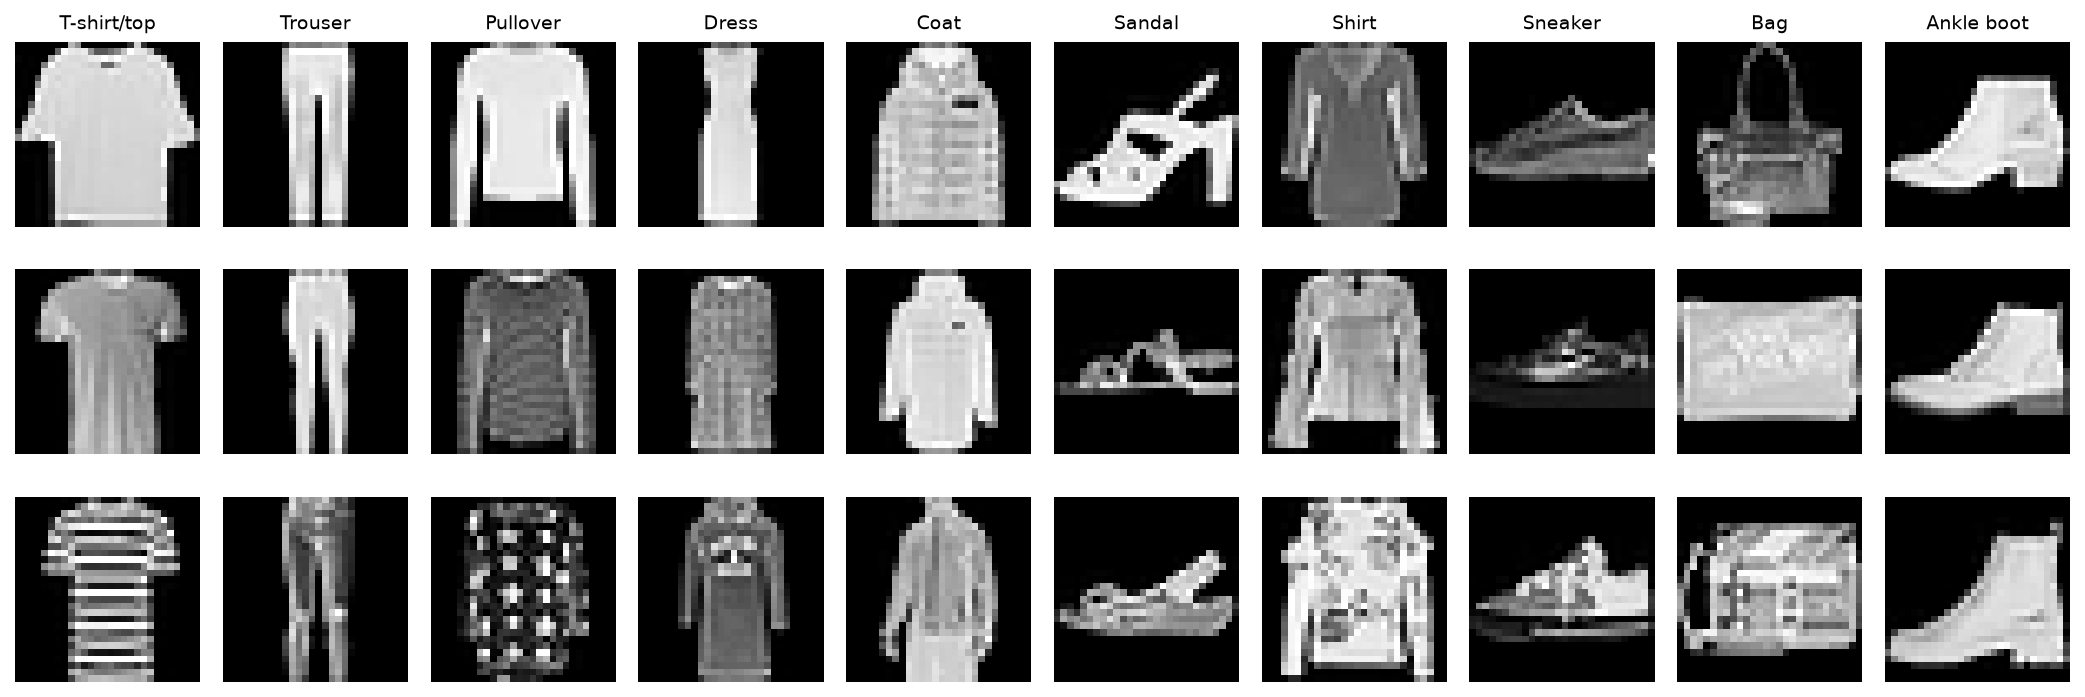
\includegraphics[width=\columnwidth]{training_samples.png}
\caption{Fixed-seed examples drawn only from the training partition.}\end{figure}
\begin{figure}[t]\centering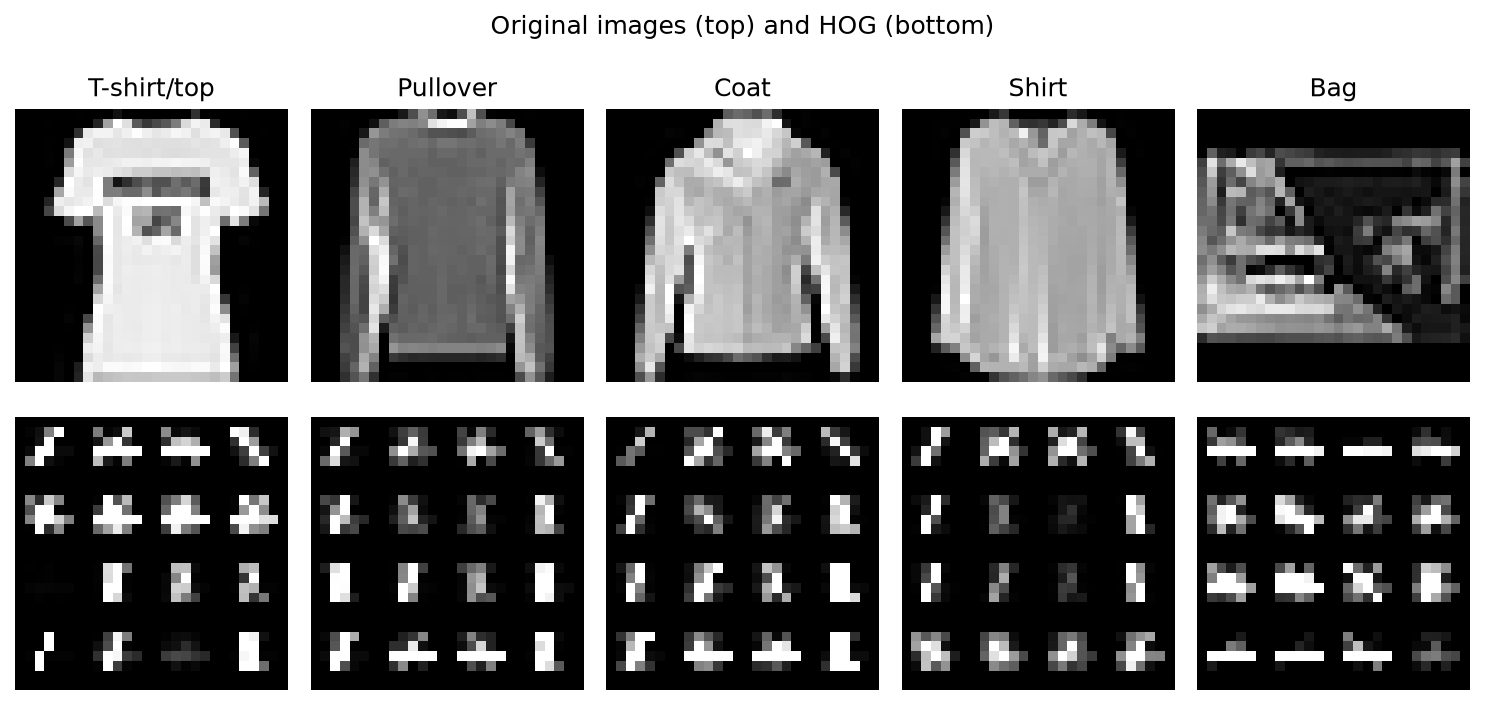
\includegraphics[width=\columnwidth]{hog_visualization.png}
\caption{Training images and HOG visualization.}\end{figure}

\section{Features and Classical Methods}
\subsection{Pixels and HOG}
Images become float32 values in $[0,1]$ after division by 255. Flattening puts all 784 values in a fixed order. Reshaping the vector recovers the image exactly. The vector classifier has no built-in local filters or weight sharing.

HOG estimates image gradients and groups their directions into histograms within cells. It normalizes overlapping blocks using L2-Hys, then joins the values into one vector. Nine bins with $7\times7$-pixel cells and $2\times2$-cell blocks give
\[d=(4-2+1)^2(2\cdot2\cdot9)=324.\]
We preserve image orientation, size, channel and labels, and apply no augmentation or segmentation.

\subsection{Decision Rules}
Logistic Regression learns regularized multiclass linear scores with probabilities proportional to $\exp(w_c^\top x+b_c)$ using log loss. Linear SVM learns margin-based one-versus-rest boundaries; $C$ controls the error/regularization tradeoff. Logistic Regression uses a StandardScaler fitted on training examples only and retained in its pipeline. Linear SVM uses the fixed normalized descriptors directly, with tolerance $10^{-3}$ and at most 2,000 iterations, to avoid amplification of rare border pixels.

Distance-weighted $k$-NN votes among nearby training vectors under Euclidean distance. Prediction requires storing and searching the training examples. Random Forest combines trees trained on bootstrap samples and random feature subsets. Neither receives a learned scaler in this experiment.

\subsection{Objectives and Hyperparameters}
For Logistic Regression, a regularized objective is
\[
-\frac{1}{n}\sum_{i=1}^n\log p_{y_i}(x_i)
+\frac{\lambda}{2}\lVert W\rVert_F^2.
\]
$C$ controls inverse regularization strength; the exact scaling of $\lambda$ depends on the library's objective convention. Larger $C$ is not guaranteed to improve generalization. For one binary one-versus-rest SVM problem, squared-hinge loss gives
\[
\tfrac12\lVert w\rVert^2+C\sum_i
\max(0,1-y_i(w^\top x_i+b))^2,
\]
where $y_i\in\{-1,+1\}$. Tolerance changes numerical stopping precision, not the model family.

Forest split quality uses Gini impurity $G=1-\sum_c p_c^2$. Bootstrap sampling and random feature subsets reduce correlation between trees; unrestricted depth can still overfit. For $k$-NN, Euclidean distance is $\sqrt{\sum_j(x_j-z_j)^2}$ and nearby examples receive greater vote weight. $k$ trades sensitivity to local examples against smoothing.

\section{Experimental Protocol}
Each core combination tests two settings: LR $C\in\{0.1,1\}$; $k$-NN $k\in\{3,5\}$; RF with (200 trees, depth 25) or (400 trees, unrestricted depth); linear SVM $C\in\{0.1,1\}$. Other settings are documented in source and recoverable from saved estimators. Convergence warnings exclude a candidate from selection.

For each combination, we select the candidate with the highest validation macro F1 and use accuracy to break ties. We use the same rule to choose the overall model. Before test evaluation, we save the choices, split, environment and hashes of the data, code and models. Evaluation does no fitting. A saved marker blocks repeat test runs in that directory, and reproduction uses a separate output directory.

Accuracy is overall correctness. For class $c$,
\[R_c=\frac{TP_c}{TP_c+FN_c},\quad
F1_c=\frac{2TP_c}{2TP_c+FP_c+FN_c},\]
and macro F1 is the unweighted mean across ten classes. Precision, recall, F1 and support are exported for every model and category. Confusion rows are true categories; columns are predictions.

\subsection{Computation and Storage}
We time every model on the same CPU with two library threads after warm-up. We repeat single-image prediction 20 times and process 1,024 images in batches of 128 over five repetitions. Timing starts with uint8 images already in memory and includes feature extraction, scaling and prediction. It excludes file decoding and model loading. We report median and p95 single-image latency separately from batch throughput.

We report linear coefficients and intercepts, tree nodes, stored examples, as appropriate for each model. These counts describe different forms of capacity and cannot be compared as equivalent parameter counts. Saved file size provides a common storage measure, though format and compression affect it.

\section{Results and Error Analysis}
Validation selects Fine HOG + RBF SVM. On the official test set, it achieves 90.87\% accuracy and macro F1 0.9084. Among the eight core models, validation selects Pixels + RF, whose test accuracy is 87.61\%. We fixed both choices before examining this experiment's test scores.
\begin{table}[t]\centering\caption{Test results using 48,000 training images. An asterisk marks an additional RBF experiment.}\label{tab:results}
\small\begin{tabular}{lrr}\toprule Model & Accuracy (\%) & Macro F1 \\ \midrule
Fine HOG + RBF SVM* & 90.87 & 0.9084 \\
Pixels + RBF SVM* & 89.73 & 0.8971 \\
Pixels + RF & 87.61 & 0.8747 \\
HOG + RBF SVM* & 87.70 & 0.8769 \\
Pixels + k-NN & 85.09 & 0.8515 \\
Pixels + LR & 83.96 & 0.8390 \\
Pixels + linear SVM & 83.97 & 0.8373 \\
HOG + LR & 84.55 & 0.8450 \\
HOG + linear SVM & 84.01 & 0.8385 \\
HOG + RF & 84.59 & 0.8455 \\
HOG + k-NN & 83.81 & 0.8382 \\
\bottomrule\end{tabular}\end{table}
\begin{figure}[t]\centering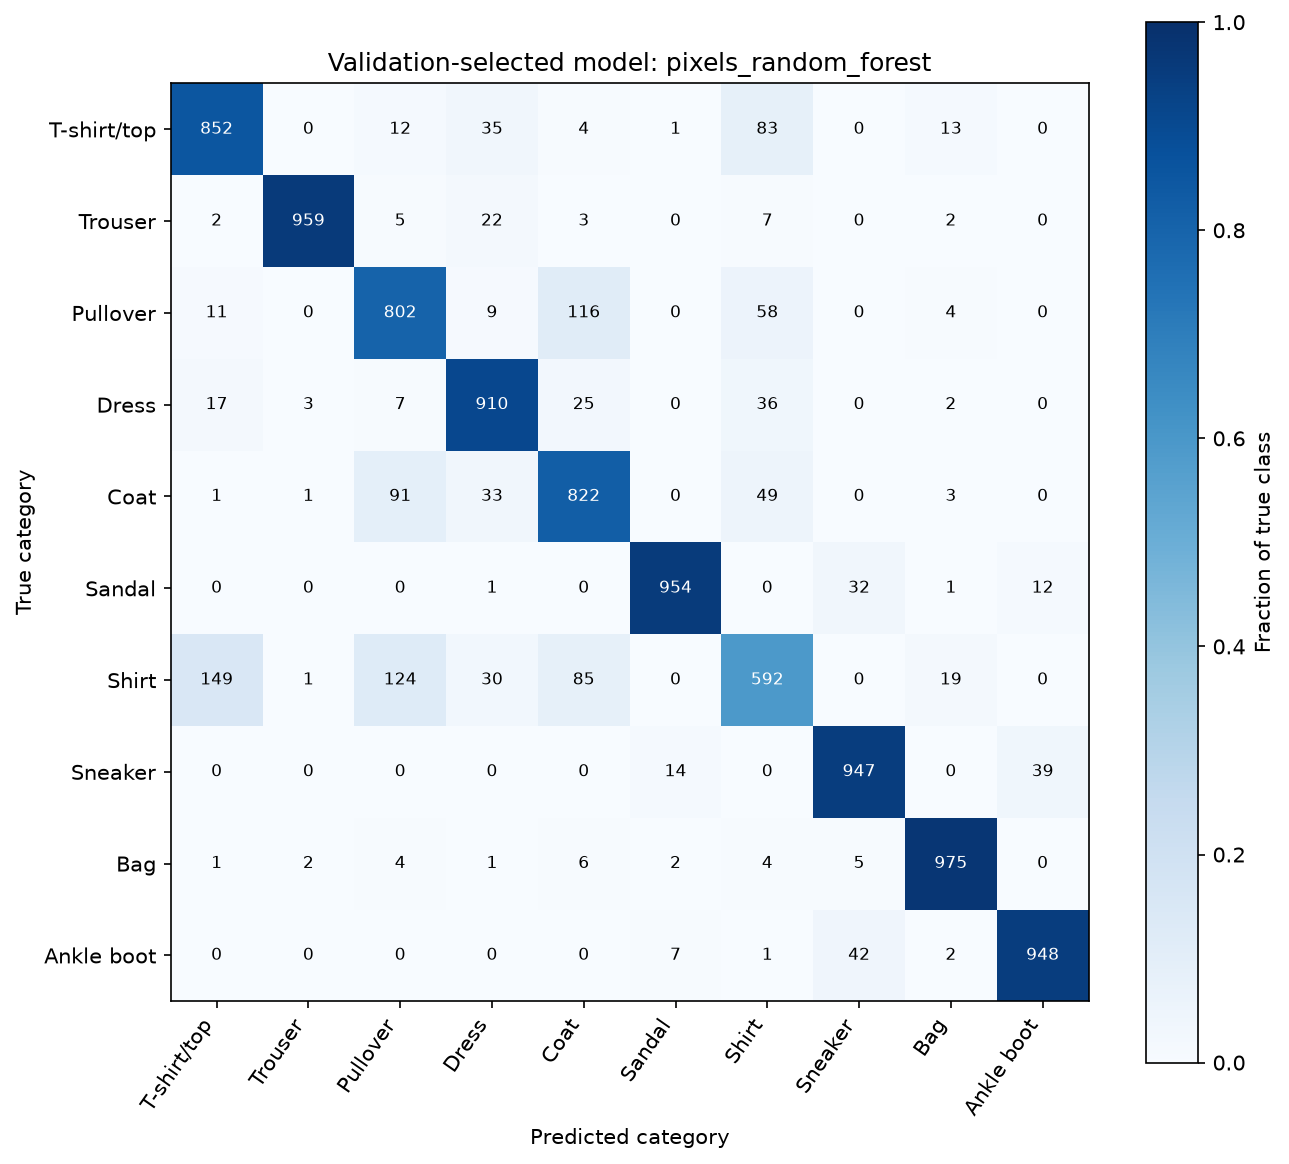
\includegraphics[width=\columnwidth]{selected_confusion.png}\caption{Official test confusion matrix for the selected model. Cells show counts, with shading normalized within each true class.}\end{figure}
\begin{table}[t]\centering\caption{Recall by category for the model selected on validation data.}\begin{tabular}{lr}\toprule Category & Recall (\%) \\ \midrule
T-shirt/top & 85.9 \\
Trouser & 97.8 \\
Pullover & 86.2 \\
Dress & 91.9 \\
Coat & 87.1 \\
Sandal & 96.7 \\
Shirt & 71.4 \\
Sneaker & 96.9 \\
Bag & 98.6 \\
Ankle boot & 96.2 \\
\bottomrule\end{tabular}\end{table}
The most frequent upper-body mistakes are Shirt to T-shirt/top: 116; T-shirt/top to Shirt: 102; Shirt to Coat: 66. Similar shapes and textures at this resolution may contribute to these errors, though we have not established the cause. The notebook includes upper-body examples sampled with a fixed seed.
The selected model uses 17,835 support vectors and 52.74 MiB of serialized storage. Median single-image latency is 10.169 ms, with p95 15.732 ms. Batch throughput is 59.5 images/s under the common protocol. These timings exclude file decoding and model loading.


\section{Reproducibility and Limitations}
The repository includes a locked \textit{uv} environment, commands for each stage, a checked notebook and tests. It records data sources and saves predictions. Datasets and fitted models are generated locally and excluded from Git. Reproduction writes to a separate directory to preserve the reported experiment. We acknowledge the supplied reference in \textit{docs/ATTRIBUTION.md}. All reported scores come from our new experiment.

We use one split and seed with a limited search, so model selection may change under other splits or settings. Optimization budgets also differ between methods. The official test set is public and appeared in the supplied reference. Our results therefore describe a familiar benchmark. We have not measured performance on phone photos, new categories, splits by product identity or near-duplicates. Blocking repeat evaluation cannot remove the risk of adapting choices to a familiar benchmark.

The reference trained on 12,000 images. We change both training size and model settings, so the accuracy difference cannot identify the effect of either change alone.

\section{Conclusion and Phase 2 Plan}
On this benchmark, the classical experiments show how pixel and HOG representations affect accuracy, category errors and prediction cost. Phase 2 should reuse the saved split for a small CNN with two or three blocks, pooling and dropout. Validation data should control early stopping. After testing architecture and regularization choices separately, we can compare CNN and classical errors on the same images. CNN performance remains to be measured.

\begin{thebibliography}{6}
\bibitem{fashion} H. Xiao, K. Rasul, and R. Vollgraf, ``Fashion-MNIST: a novel image dataset for benchmarking machine learning algorithms,'' arXiv:1708.07747, 2017.
\bibitem{hog} N. Dalal and B. Triggs, ``Histograms of oriented gradients for human detection,'' in \emph{CVPR}, vol. 1, pp. 886--893, 2005.
\bibitem{svm} C. Cortes and V. Vapnik, ``Support-vector networks,'' \emph{Machine Learning}, vol. 20, pp. 273--297, 1995, doi:10.1007/BF00994018.
\bibitem{rf} L. Breiman, ``Random forests,'' \emph{Machine Learning}, vol. 45, pp. 5--32, 2001, doi:10.1023/A:1010933404324.
\bibitem{knn} T. Cover and P. Hart, ``Nearest neighbor pattern classification,'' \emph{IEEE Trans. Inf. Theory}, vol. 13, no. 1, pp. 21--27, 1967.
\bibitem{cnn} Y. LeCun, L. Bottou, Y. Bengio, and P. Haffner, ``Gradient-based learning applied to document recognition,'' \emph{Proc. IEEE}, vol. 86, no. 11, pp. 2278--2324, 1998.
\end{thebibliography}
\end{document}
